
\subsection{Work Breakdown Structure}

\tikzset{
	basic/.style  = {draw, text width=2cm, font=\sffamily, rectangle},
	root/.style   = {basic, rounded corners=2pt, thin, align=center,
		fill=green!30},
	level 2/.style = {basic,sibling distance=15mm, rounded corners=6pt, thin,align=center, fill=green!60,
		text width=6em},
	level 3/.style = {basic, thin, align=left, fill=red!40, text width=6em},
	level 4/.style = {basic, thin, align=left, fill=red!20, text width=8em}
}

\tikzset{
	basic/.style  = {draw, text width=2cm, font=\sffamily, rectangle},
	root/.style   = {basic, rounded corners=2pt, thin, align=center,
		fill=green!30},
	level 2/.style = {basic,sibling distance=15mm, rounded corners=6pt, thin,align=center, fill=green!60,
		text width=6em},
	level 3/.style = {basic, thin, align=left, fill=red!40, text width=6.5em},
	level 4/.style = {basic, thin, align=left, fill=red!20, text width=8em}
}

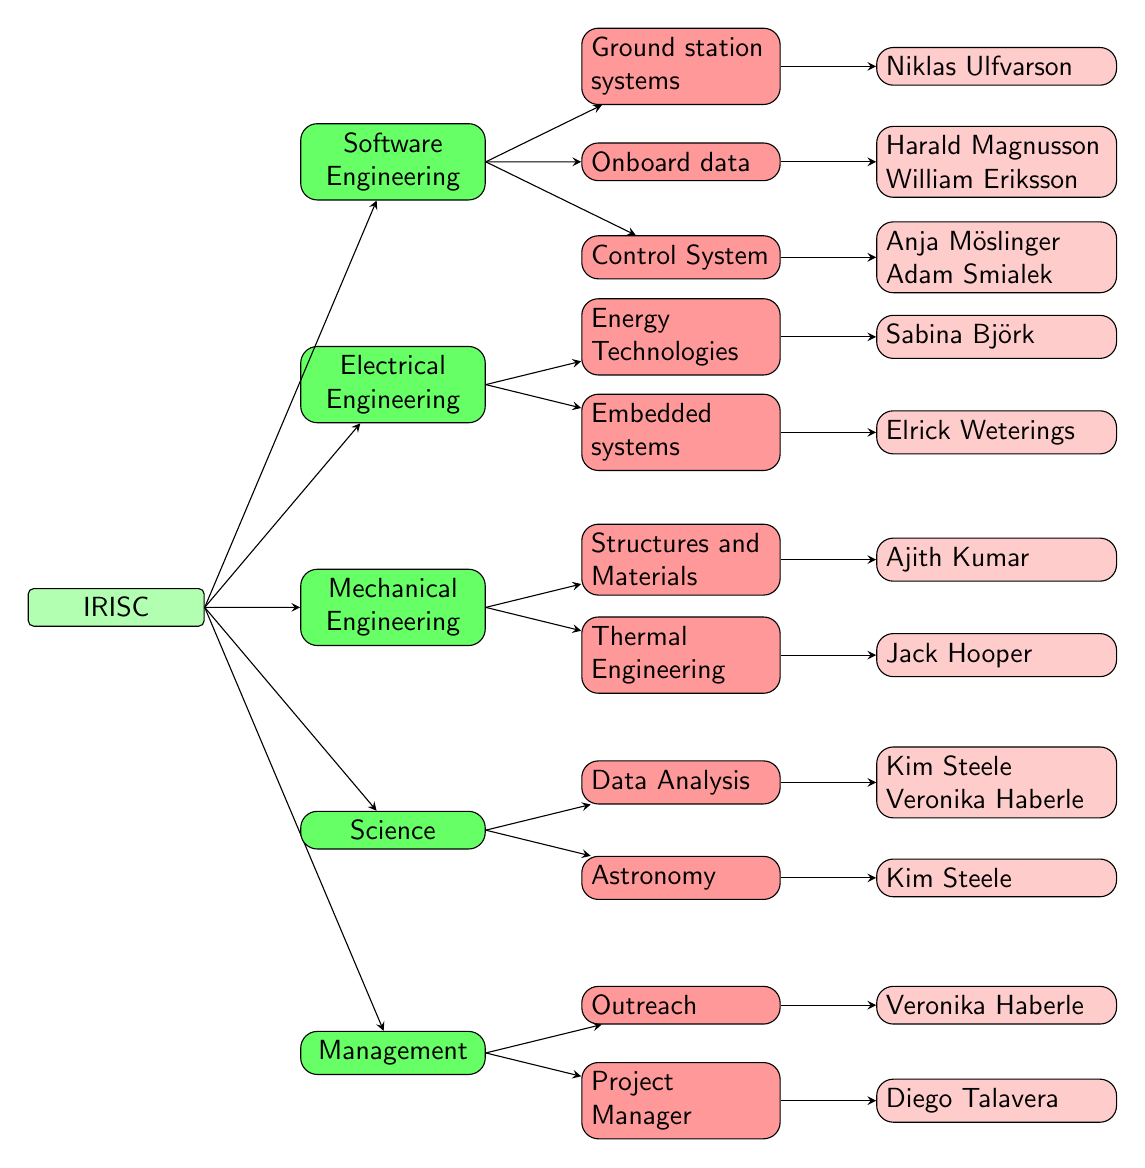
\begin{tikzpicture}[grow=right, , anchor=west, growth parent anchor=east, parent anchor=east, scale=\textwidth/15cm,
level 1/.style={sibling distance=35mm}, edge from parent/.style={->,draw},
>=stealth]

% root of the the initial tree, level 1
\node[root] {IRISC}
% The first level, as children of the initial tree
child {node[level 2] (c1) {Management}
	child{node[level 3] (c11){Project \\ Manager}
		child{node[level 4](c111){Diego Talavera}}
	}
	child{node[level 3] (c12){Outreach}
		child{node[level 4](c121){Veronika Haberle}}
	}
}
child {node[level 2] (c2) {Science}
	child {node [level 3] (c21) {Astronomy}
		child{node[level 4](c211){Kim Steele}}
	}
	child {node [level 3] (c22) {Data Analysis}
		child{node[level 4](c221){Kim Steele \\ Veronika Haberle}}
	}
}
child {node[level 2] (c3) {Mechanical Engineering}
	child {node [level 3](c31) {Thermal \\ Engineering}
		child{node[level 4](c311){Jack Hooper}}
	}
	child {node [level 3](c32) {Structures and Materials}
		child{node[level 4](c321){Ajith Kumar}}
	}
}
child {node[level 2] (c4) {Electrical Engineering}
	child {node [level 3] (c41) {Embedded \\ systems}
		child{node[level 4](c411){Elrick Weterings}}
	}
	child {node [level 3] (c42) {Energy \\ Technologies}
		child{node[level 4](c421){Sabina Bj{\"o}rk}}
	}
}
child {node[level 2] (c5) {Software Engineering}
	child {node [level 3] (c51) {Control System}
		child{node[level 4](c511){Anja M{\"o}slinger \\ Adam Smialek}}
	}
	child {node [level 3] (c52) {Onboard data}
		child{node[level 4](c521){Harald Magnusson \\ William Eriksson}}
	}
	child {node [level 3] (c53) {Ground station systems}
		child{node[level 4](c531){Niklas Ulfvarson}}
	}
};

\end{tikzpicture}
The IRISC team is divided in 5 major branches: Management, Science, Mechanical Engineering, Electrical Engineering an Software Engineering. Diego Talavera will also work in the Mechanical Engineering branch whenever needed. The Electrical and Software Engineering branches will work closely together to achieve a correct integration between hardware and software.
